% !TeX document-id = {2dbf9b71-bbba-4dd9-bbd6-409e1a74ac36}
% !TeX TXS-program:compile = txs:///pdflatex/[--shell-escape] | txs:///biber | txs:///pdflatex/[--shell-escape]
\documentclass[spanish,utf8]{beamer}
\usepackage[T1]{fontenc}
\usepackage[spanish]{babel}
\usepackage{amsmath,mathrsfs,amsfonts,amsthm}
\usepackage{caption}
%\usepackage[figurename=Figura]{caption}
\usepackage[backend=biber,style=numeric, defernumbers=true, sorting=ynt]{biblatex}
\addbibresource{bibliography/reference.bib}
%% Fix so biblatex works instead of natbib
\makeatletter
\let\c@author\relax
\makeatother
\let\bibhang\relax
\let\citename\relax
\let\bibfont\relax
\let\Citeauthor\relax
\expandafter\let\csname ver@natbib.sty\endcsname\relax

%% Fix headers and footers
\makeatletter
\def\ps@pprintTitle{%
	\let\@oddhead\@empty
	\let\@evenhead\@empty
	\def\@oddfoot{\centerline{\thepage}}%
	\let\@evenfoot\@oddfoot}
\makeatother

%% Load some packages and stuff
%\usepackage[backend=biber,style=numeric, defernumbers=true, sorting=ynt,maxbibnames=4,maxcitenames=4]{biblatex}
%% Library and stuff
\usepackage[style=numeric,sortcites=true,sorting=ynt,backend=biber]{biblatex}
%% biblatex med apa-style. Det vivill ha
\DeclareLanguageMapping{american}{american-apa} %% Vi vill ha svensk apa
\bibliography{../bibliography/reference}

\usepackage[T1]{fontenc}
\usepackage[spanish]{babel}
\usepackage{pifont}
\usepackage{geometry}
\usepackage[svgnames]{xcolor}
\usepackage{graphicx}
\usepackage{sagetex}
\usepackage{minted}
\usepackage{float}
\usepackage{tkz-graph}
\usepackage{txfonts}
\usepackage{amsmath,amsthm}
\theoremstyle{definition}
\usepackage{bm}
\usepackage[colorlinks=true,urlcolor=blue,linkcolor=black,anchorcolor=black,citecolor=black]{hyperref}
\hypersetup{pdfinfo={
		Title={El teorema de los cuatro colores},
		Author={Grupo Nº6},
		Keywords={teorema de los cuatro colores, cadena de Kempe, grafos planares, coloración de mapas},
		Subject={Introducción a la matemática discreta},
		Producer={TeXstudio 2.12.8},
		Creator={pdfTeX Version 3.14159265 TeX Live 2018 Debian}
}}


\usepackage{etoolbox}
\AtBeginDocument{%
	%\patchcmd{<cmd>}{<search>}{<replace>}{<success>}{<failure>}
	%\patchcmd{\ps@pprintTitle}% <cmd>
	%{Preprint submitted}% <search>
	%{To be submitted}% <replace>
	%{}{}% <succes><failure>
	\patchcmd{\MaketitleBox}{\vspace*{-20pt}\fi}{\fi}{}{}%
	\patchcmd{\abstract}{Abstract}{Resumen}{}{}
	\patchcmd{\keyword}{Keywords}{Palabras clave}{}{}
}

%\makeatletter
%\patchcmd{\ps@pprintTitle}{\footnotesize\itshape
%	Preprint submitted to \ifx\@journal\@empty Elsevier
%	\else\@journal\fi\hfill\today}{\relax}{}{}
%\makeatother

\makeatletter
\def\printFirstPageNotes{%
	\iflongmktitle
	\let\columnwidth=\textwidth\fi
	\ifx\@tnotes\@empty\else\@tnotes\fi
	\ifx\@nonumnotes\@empty\else\@nonumnotes\fi
	\ifx\@cornotes\@empty\else\@cornotes\fi
	\ifx\@elseads\@empty\relax\else
	\let\thefootnote\relax
	\footnotetext{\ifnum\theead=1\relax
		\textit{Correo electrónico:\space}\else
		\textit{Correos electrónicos:\space}\fi
		\@elseads}\fi
	\ifx\@elsuads\@empty\relax\else
	\let\thefootnote\relax
	\footnotetext{\textit{Sitio web:\space}%
		\@elsuads}\fi
	\ifx\@fnotes\@empty\else\@fnotes\fi
	\iflongmktitle\if@twocolumn
	\let\columnwidth=\Columnwidth\fi\fi
}
\makeatother

%% `Elsevier LaTeX' style
%\bibliographystyle{elsarticle-num}
\renewcommand{\spanishcontentsname}{Tabla de contenidos}
\renewcommand{\spanishfigurename}{Fig.}
\renewcommand{\listingscaption}{Programa}
%\newcommand{\MVAt}{{\usefont{U}{mvs}{m}{n}\symbol{`@}}}
\newtheorem{definition}{Definición}
\newtheorem{example}{Ejemplo}
\newtheorem{theorem}{Teorema}

\graphicspath{{../images/}}
\theoremstyle{definition}
%\newtheorem{theorem}{Teorema}[section]
%\newtheorem{definition}{Definición}
\newtheorem{remark}{Observación}

\usetheme{CambridgeUS}
\usecolortheme{dolphin}
\useinnertheme{rectangles}
%\useoutertheme[hooks]{tree}

\usefonttheme[onlymath]{serif}

\setbeamercovered{transparent}

\setbeamertemplate{footline}[frame number]{}
\setbeamertemplate{navigation symbols}{}
\setbeamertemplate{footline}{}
\setbeamertemplate{headline}{}

\title[Teorema de los cuatro colores]{\Huge\sffamily El teorema de los cuatro colores}
\subtitle{Introducción a la matemática discreta CM -- 254}

\author[Grupo N$^\circ6$]{%
	\texorpdfstring{%
		\begin{columns}
			\column{.3\linewidth}
			\centering
			C. Aznarán Laos %\inst{1,2}
			\column{.3\linewidth}
			\centering
			F. Cruz Ordoñez %\inst{1,2}
		\end{columns}
		\vspace{12pt}
		\begin{columns}
			\column{.3\linewidth}
			\centering
			G. Quiroz Gómez %\inst{1,2}
			\column{.3\linewidth}
			\centering
			J. Navío Torres %\inst{1,2}
		\end{columns}
	}
	{Author 1, Author 2, Author 3}
}

\institute[FC -- UNI]{\large%\inst{1}
	Facultad de Ciencias \and%\inst{2}
	Universidad Nacional de Ingeniería
}
\date{18 de junio del 2018}

%\usetheme{Warsaw}
%\usetheme{Pittsburgh}
%\usetheme{Rochester}
%\usetheme{EastLansing}
%\usetheme{Frankfurt}
%\usetheme{default}
%\usetheme{Bergen}
%\usetheme{Boadilla}
\graphicspath{{images/}}

\AtBeginSubsection[]
{
	\begin{frame}<beamer>
	\frametitle{\contentsname}
	\tableofcontents[
	currentsection,
	sectionstyle=show/show,
	subsectionstyle=show/shaded/hide
	]
\end{frame}
}

\begin{document}

\begin{frame}[plain]
\maketitle
\end{frame}

\section{Introducción}

\begin{frame}{\contentsname}\transblindsvertical
\tableofcontents
\end{frame}

\subsection{El problema de los cuatro colores}


\begin{frame}{\insertsubsection}\transblindsvertical

\begin{alertblock}{Pregunta} % 1852 Francis Guthrie
	¿Es posible colorear cualquier mapa geográfico plano usando solamente \emph{cuatro colores}, de modo que dos países con frontera común tengan colores diferentes? 
\end{alertblock}

\begin{minipage}[c]{6cm}
	\begin{figure}
		\centering
		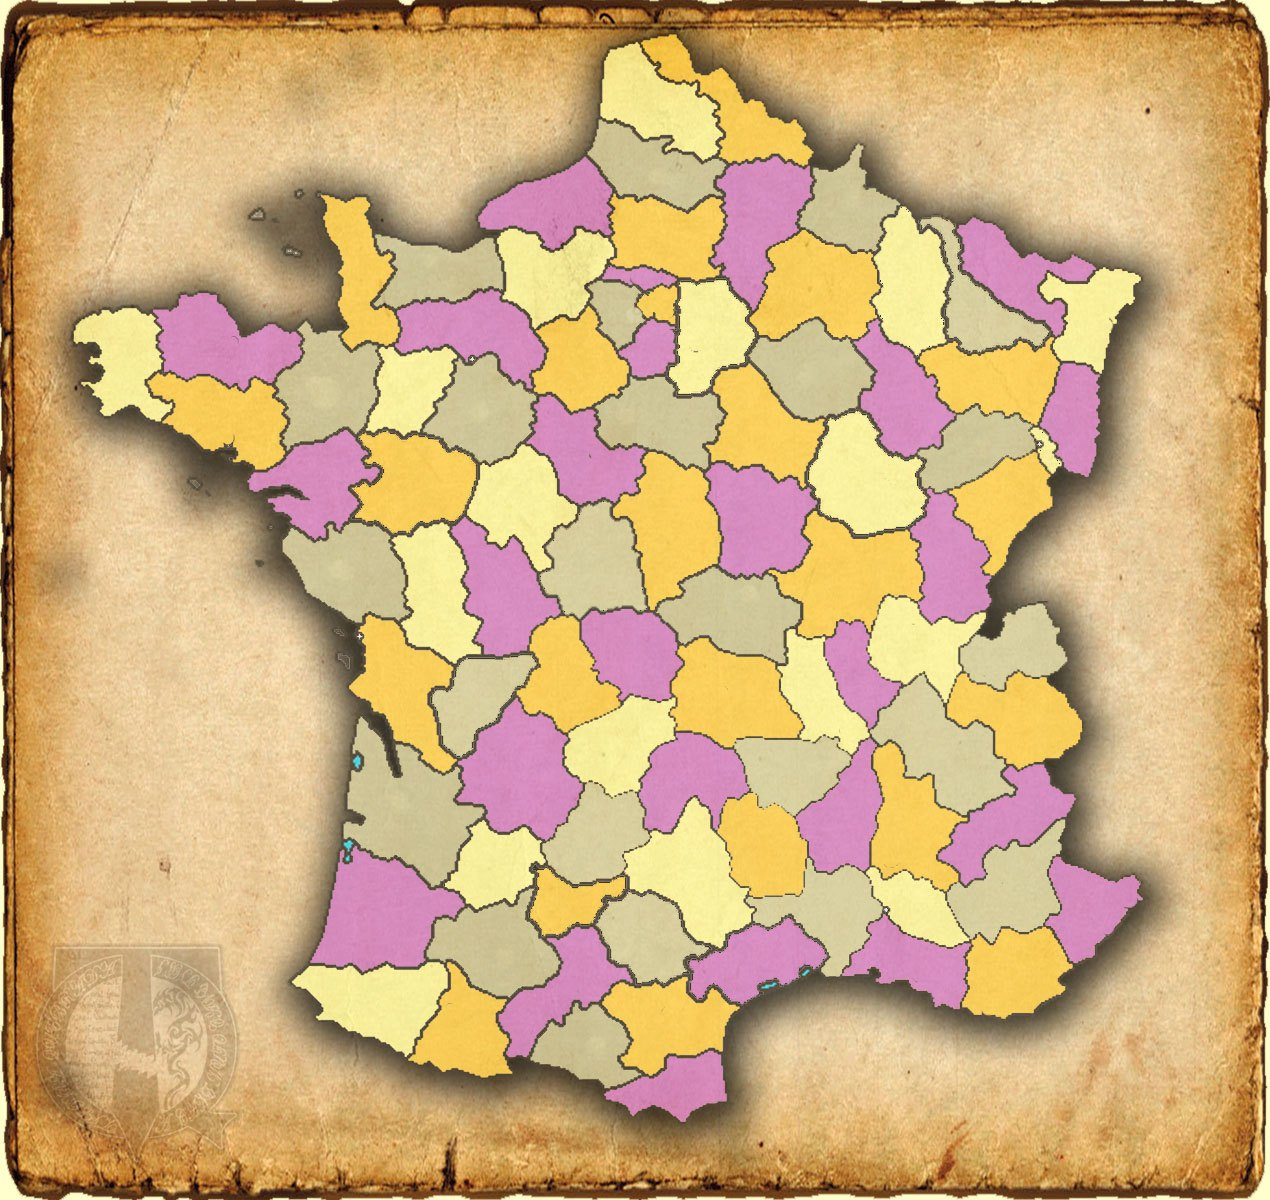
\includegraphics[width=4cm]{mapa-4-colores_HR.jpg}
		\caption{Mapa político coloreado}
	\end{figure}
\end{minipage}
\begin{minipage}[c]{5cm}
	\begin{definition}[Mapa conexo]
		Un mapa es conexo\footnote{de una pieza} y cada una de sus regiones también es conexa.
	\end{definition}
\end{minipage}
\end{frame}

{
	\usebackgroundtemplate{\centering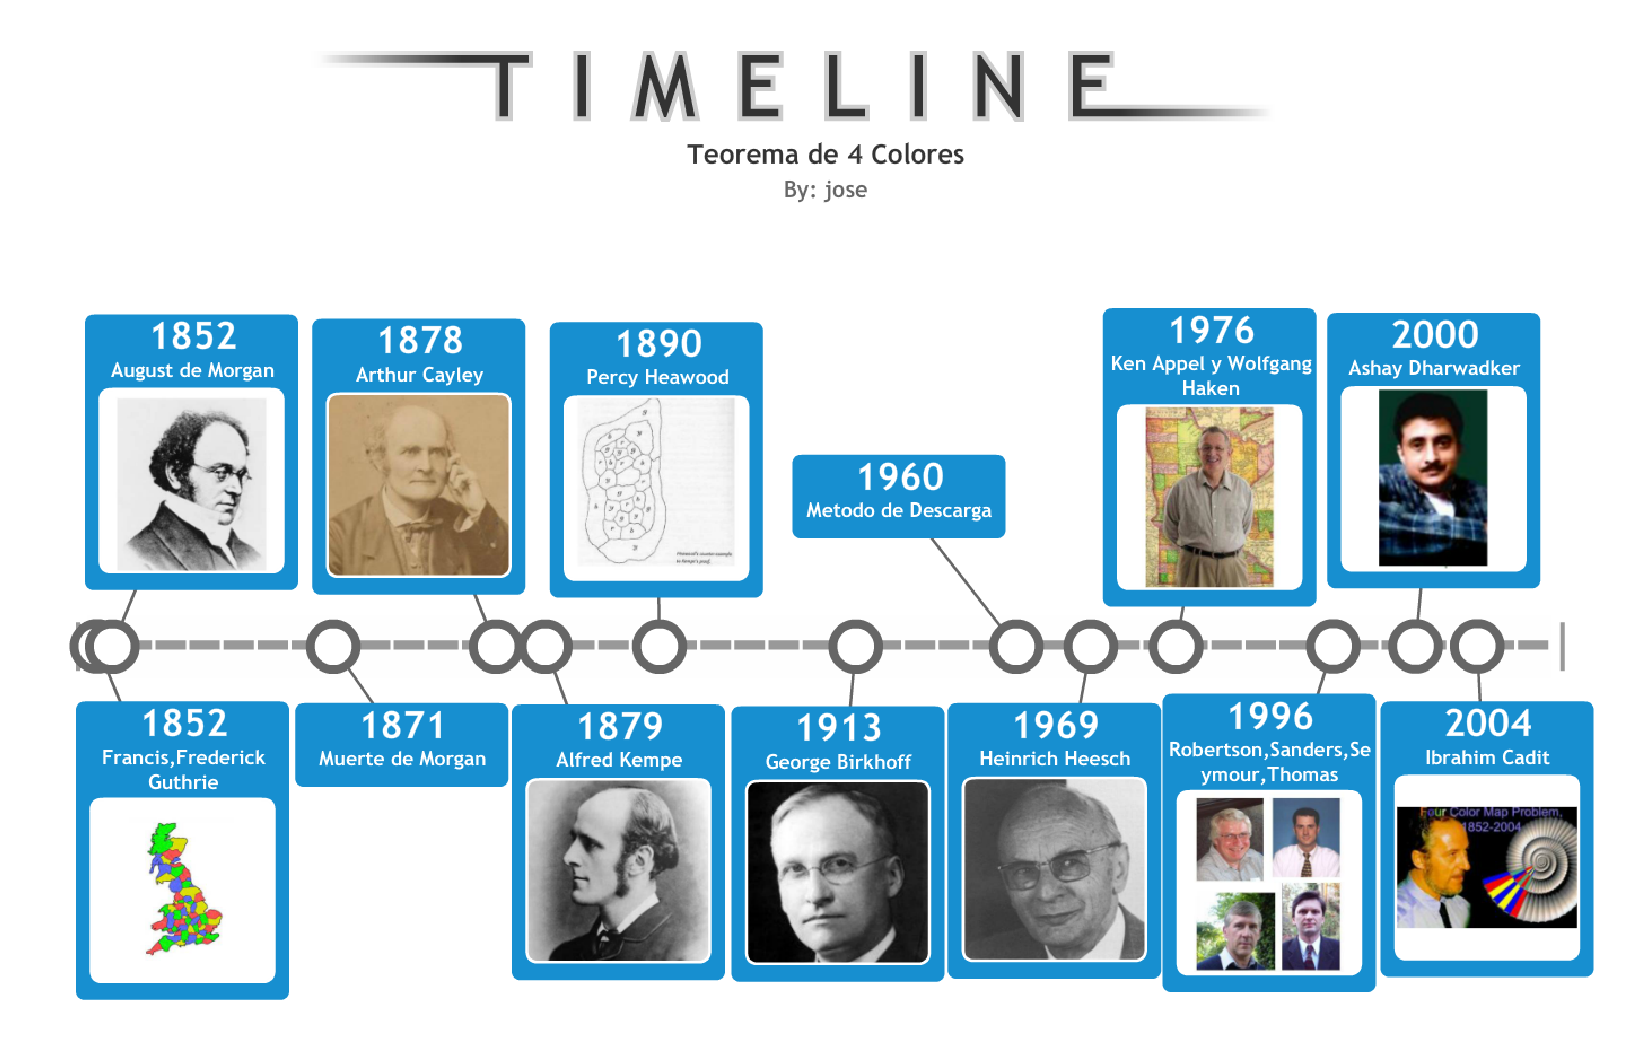
\includegraphics[width=\paperwidth]{crop}}%height=\paperheight,
	\begin{frame}[plain]
\end{frame}
}

\section{Un poco de historia}

\subsection{Formulación de la conjetura}

\begin{frame}{\insertsection}\transblindsvertical
\begin{flushright}
	\begin{block}{Francis Guthrie (1839-1899)}
		Abogado y botánico, observa que puede colorear un mapa complejo de los cantones de Inglaterra con 4 colores. En 1852, enuncia el problema a su hermano Frederick (University College London) y a éste a Augustus de Morgan. Francis Guthrie observa que 3 colores no son suficientes, con el diagrama crítico:
	\end{block}
	\begin{figure}
		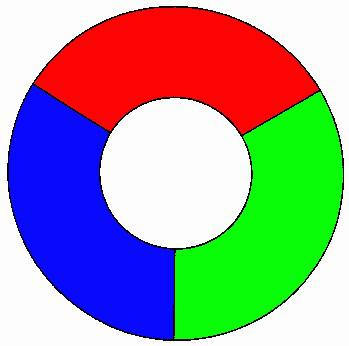
\includegraphics[scale=0.3]{diagrama.jpg}
		\caption{Diagrama Crítico}
	\end{figure}
\end{flushright}
\end{frame}

\begin{frame}{\insertsubsection}
\begin{remark}{}
	Dos regiones no pueden tocarse solo en un punto, y así, se pueden ignorar regiones con una única línea frontera.
\end{remark}
\begin{center}
	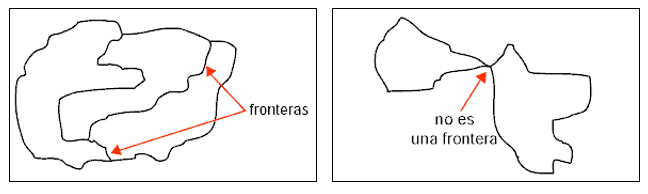
\includegraphics[height=3cm]{fronteras.png}
\end{center}

Es un problema topológico: no importa la forma de las regiones, sino como están colocadas unas respecto a otras.
\end{frame}

\begin{frame}{\insertsubsection}\transblindsvertical
Leonhard Euler
\begin{theorem}[Fórmula de Euler para mapas]
	$$
	\#\text{caras} - \#\text{aristas} + \#\text{vértices} = 2.
	$$
\end{theorem}
\begin{center}
	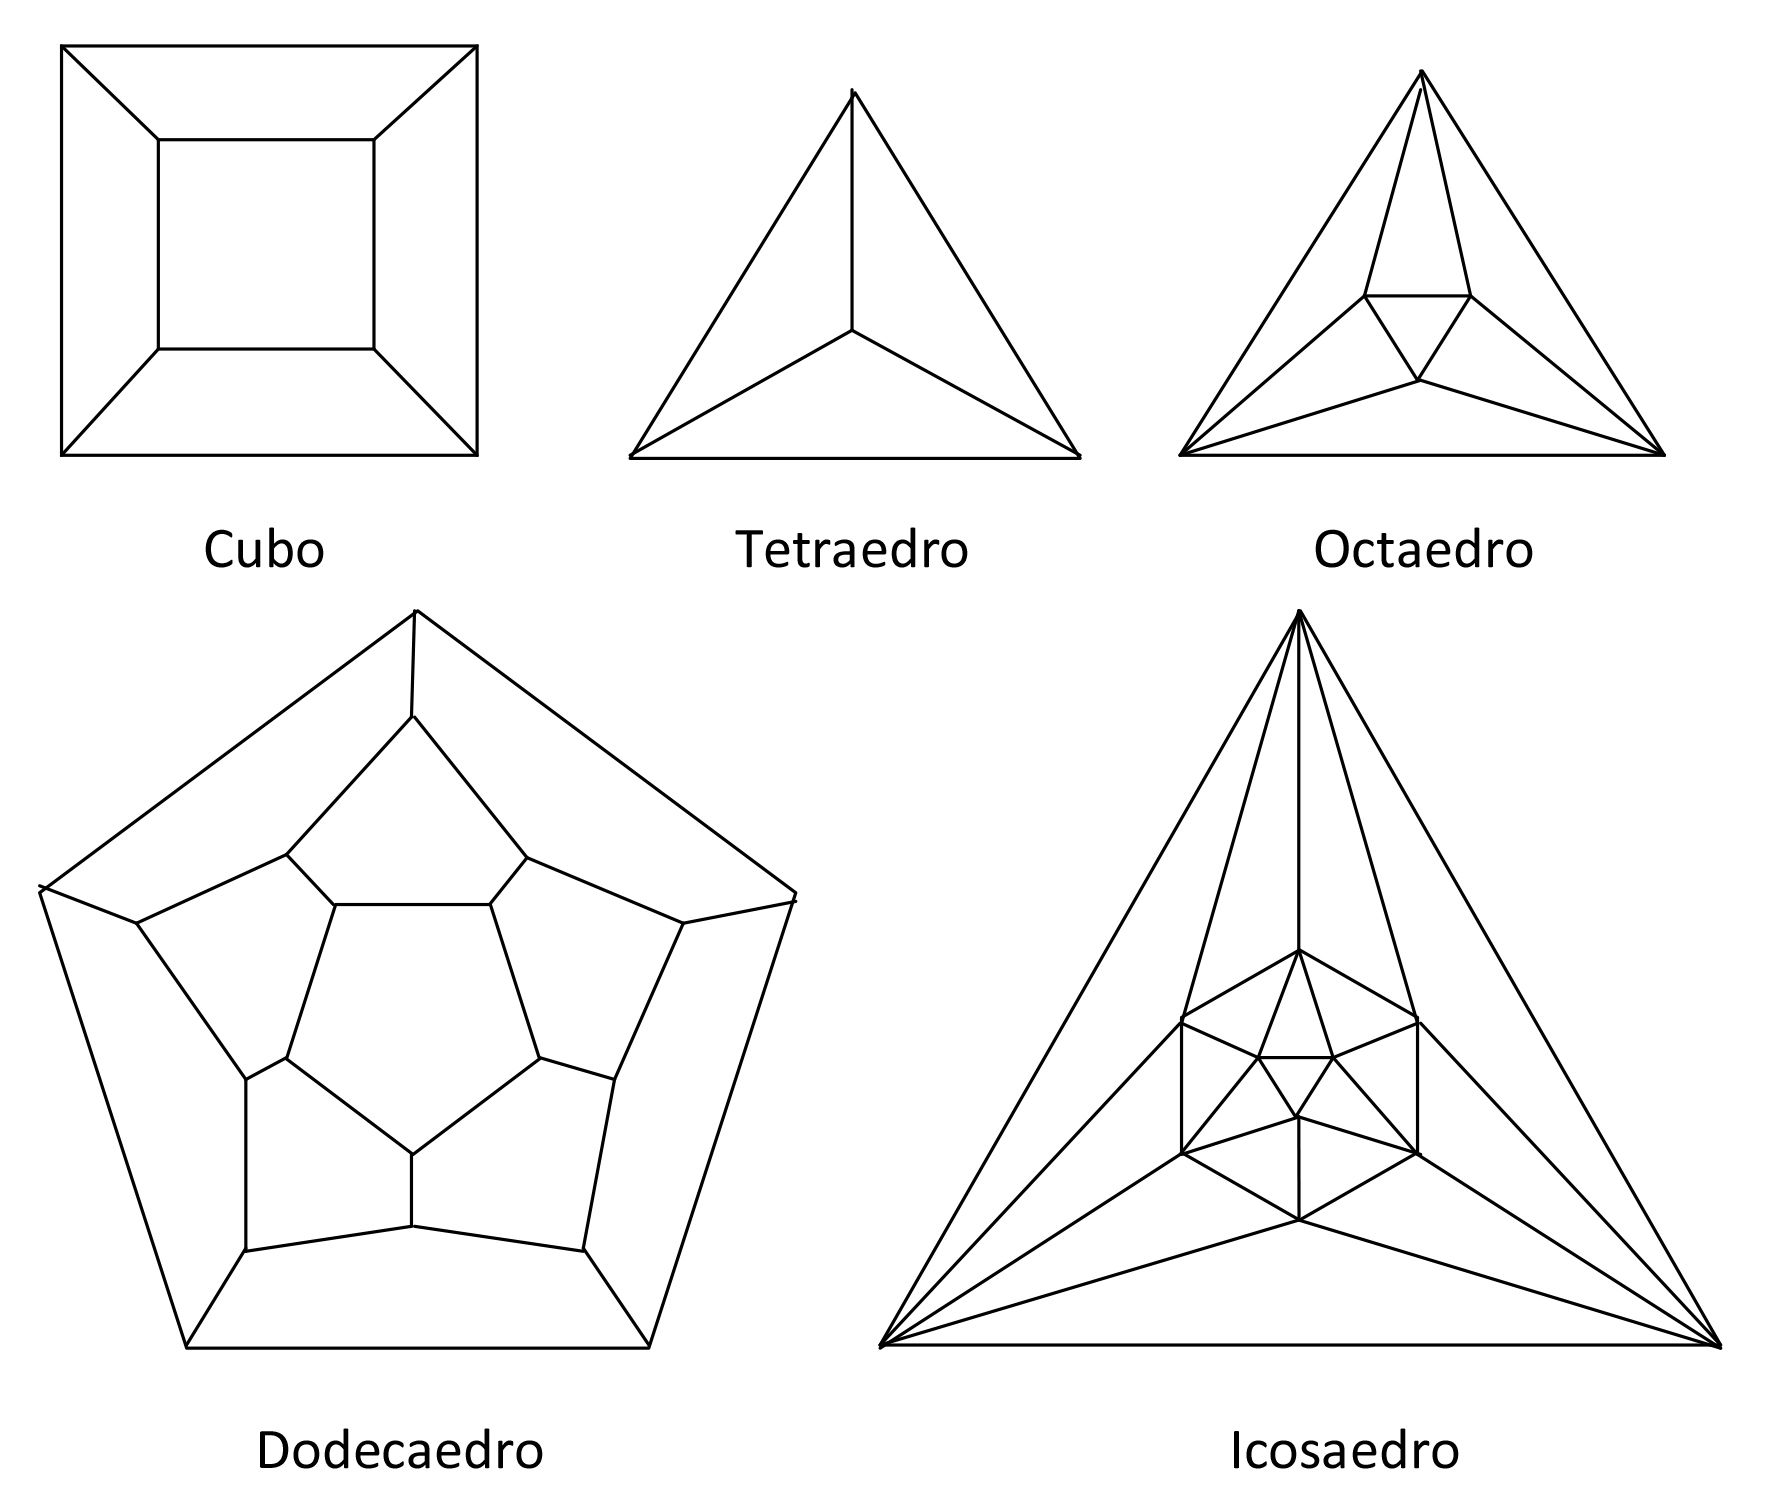
\includegraphics[height=5cm]{poliedros2.jpg}
\end{center}
\end{frame}

\subsection{Primer intento de demostración: Las cadenas de \citeauthor{kempe}}

\subsection{El error fatal de \citeauthor{kempe} por Heawood}

\subsection{Algunas definiciones más}

\begin{frame}[allowframebreaks]
\frametitle{\insertsubsection}

\begin{definition}[Número cromático] 
Sea $G=(V,E)$ un grafo y sea $k$ un número natural. Una aplicación $c:V\to \{1,2,\ldots k\}$ se llama \emph{coloración del grafo} $G$ si $c(x)\neq c(y)$ se cumple para cada rama $\{x,y\}\in E$. \linebreak El número cromático de $G$, denotado por $x(G)$, es el \emph{mínimo valor} de $k$ para el cual existe una coloración $c:V(G)\to {1,2\ldots,k}$.
\end{definition}

\begin{definition}[Grafo Dual]
Sea $G=(V,E)$ un grafo planar con un dibujo planar fijo. Denotamos $\mathcal{F}$ por el conjunto de caras de $G$. Definimos un grafo, con posibles lazos y ramas múltiples, como $(\mathcal{F},E,\epsilon)$, donde $\epsilon$ se define como $\epsilon(e)={F_i,F_J]}$ siempre que la rama $\epsilon$ sea una frontera común de las caras $F_i,F_j$ (también permitimos que $F_i=F_j$, en el caso en que la misma cara este ambos lados de una rama dada).

Este grafo $(\mathcal{F},E,\epsilon)$ se le llama el dual (\emph{geométrico}) de $G$ y se denota por $G^*$.	
\end{definition}
\end{frame}

\subsection{Algunos ejemplos}

\begin{frame}[allowframebreaks]
\frametitle{\insertsubsection}

\begin{example}[Ejemplo de Grafos Duales]
Para construir una gráfica dual de un grafo plano $G$ se debe colocar un vértice dentro de cada región de $G$ e incluir la región infinita de $G$. Para cada arista compartida por las $2$ regiones, se debe dibujar una arista que conecte a los vértices dentro de estas regiones y para cada arista que se recorre $2$ veces en el camino cerrado alrededor de las aristas de una región se dibuja un lazo en el vértice de la región. 
\end{example}

\begin{figure}[H]
	\captionsetup{justification=centering,margin=0.5cm}
	\centering
	\begin{minipage}{.5\textwidth}
		\centering
		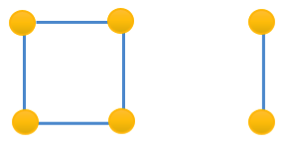
\includegraphics[width=3cm]{example1.png}
		\caption{Grafo $G$.}
	\end{minipage}%
	\begin{minipage}{0.5\textwidth}
		\centering
		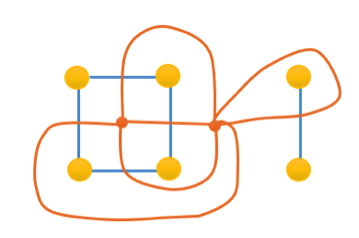
\includegraphics[width=3cm]{example2.png}
		\caption{Grafo $G$ y su dual $G^{\ast}$.}
	\end{minipage}
\end{figure}

\begin{example}[Otro ejemplo]
Sea $G=(V,E)$ un grafo plano, se llama grafo dual de $G$ y se denota por $G^{\ast}$, aquel construido de la siguiente manera:

\begin{enumerate}
	\item Se elige un punto $v_i$ en cada cara $F_i$ de $G$. Estos puntos son los vértices de $G^{\ast}$.

	\item Por cada arista $e\in E$ se traza una línea $e^{\ast}$ que atraviesa únicamente la arista $e$, y se unen los vértices $v_i$ pertenecientes a las caras adjuntas a $e$. Estas líneas son las aristas de $G^{\ast}$. A continuación se ilustra este procedimiento de construcción con un ejemplo:
	\end{enumerate}
\end{example}

\begin{figure}[H]
	\captionsetup{justification=centering,margin=0.5cm}
	\centering
	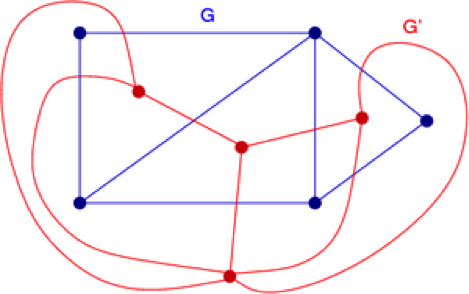
\includegraphics{example3.png}
	\caption{Grafo planar $G$ y	su grafo dual $G^{\prime}=G^{\ast}$.}
\end{figure}

\end{frame}

\subsection{Idea clave: La reducibilidad de mapas de \citeauthor{birkhoff}}

\begin{frame}
\frametitle{\insertsection:\insertsubsection}
\begin{theorem}[\citeauthor{birkhoff}]
\begin{enumerate}
	\item La conjetura de los cuatro colores puede ser falsa.
	
	\item Es posible hallar una colección finita de configuraciones reducibles tal que cualquier mapa planar debe contener uno de ellos (lo que probaría la conjetura de cuatro colores)
	
	\item la conjetura de cuatro colores puede ser cierta, pero pueden requerirse métodos más complicados para una prueba
\end{enumerate}
\end{theorem}
\end{frame}

\subsection{Demostración de \citeauthor{appel}}

\subsubsection{Método de descarga}
\subsubsection{Método de reducibilidad}

\subsection{Demostración de \citeauthor{robertson}}

%\begin{frame}{Personajes}
%\centering
%\begin{minipage}[c]{3cm}
%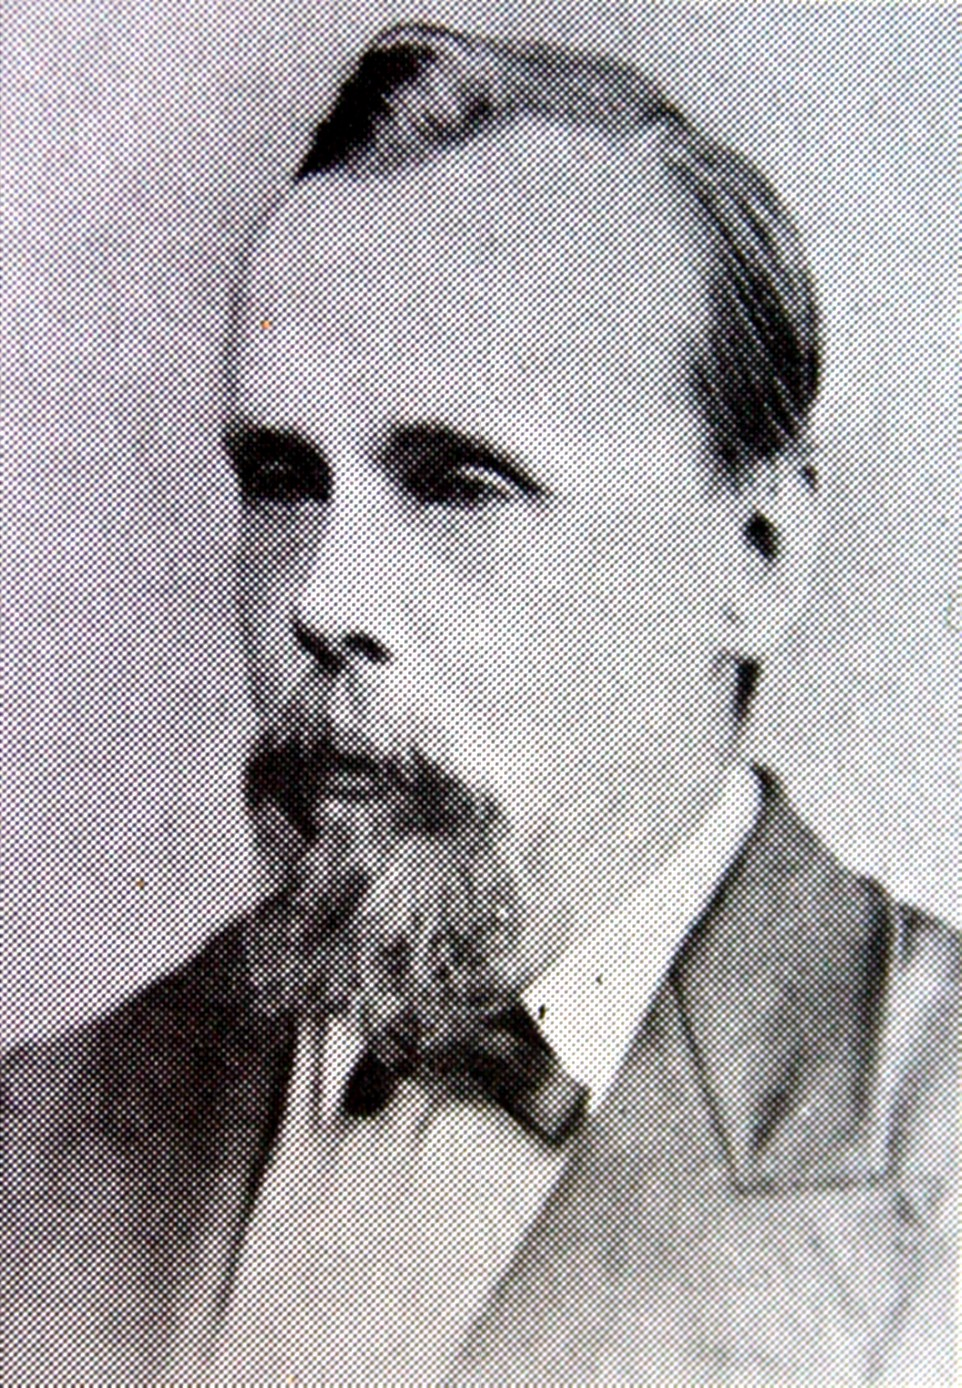
\includegraphics[width=2.5cm]{Francis_guthrie} \\
%\centering \bf{FRANCIS GUTHRIE}
%\end{minipage}
%\begin{minipage}[c]{4cm}
%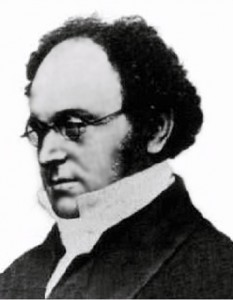
\includegraphics[width=2.5cm]{morgan.jpg}\\
%\centering\bf{AUGUST DE MORGAN}
%\end{minipage}
%\begin{minipage}[c]{3cm}
%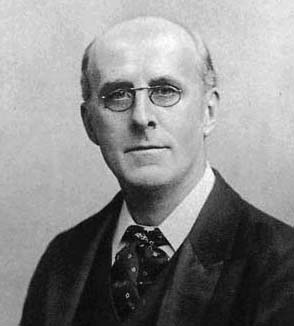
\includegraphics[width=2.5cm]{kempe.jpeg}\\
%\centering\bf{ALFRED BRAY KEMPE}
%\end{minipage}
%\end{frame}

\begin{frame}{\insertsection}\transblindsvertical
Fechas importantes
\begin{itemize}
    \item 1852: Francis Guthrie plantea el problema a su hermano Frederick y éste a Augustus de Morgan.
    
    \item  1878: Arthur Cayley publica el enunciado de la conjetura.
    
    \item  1879: Sir Alfred Bray Kempe publica su demostración.
    
    \item  1913: George Birkhoff introduce la noción de configuración reducible.
    
    \item  1960: Se introduce el llamado método de descarga.
    
    \item  1969: Avances de Heinrich Heesch en reducibilidad y obtención de conjuntos inevitables de configuraciones.
    
    \item 1976: Ken Appel y Wolfgang Haken prueban con ayuda de un ordenador que sus 1.482 configuraciones son reducibles (50 días de cálculo).
    
    \item  1996: N. Robertson, D.P. Sanders, P. Seymour y R. Thomas mejoran la demostración con ayuda de ordenador (sólo 633 configuraciones) y automatizan la prueba de la inevitabilidad.
\end{itemize}   
\end{frame}

\begin{frame}{\insertsection}\transblindsvertical
August de Morgan
\begin{block}{Difusión del teorema}
Augustus de Morgan (1806-1871) estaba muy interesado en la conjetura de los 4 colores y difundió entre sus colegas su importancia. Una de las primeras personas con las que ``habló'' fue con el matemático y físico irlandés Sir William Rowan Hamilton (1805-1865), que no compartía el interés de De Morgan por el problema. Le escribe una carta el 23 de octubre de 1852.
\end{block}

\begin{block}{Respuesta de Hamilton}
Cuatro días después, Hamilton le contesta: ``I am not likely to attempt your “quaternion” of colours very soon''.
\end{block}    
\end{frame}

\begin{frame}{\insertsection}\transblindsvertical
\begin{block}{Primera demostración}
Kempe se interesa por el problema de los 4 colores tras la pregunta de Cayley en la London Mathematical Society.
\end{block}

\begin{block}{}
En junio de 1879 obtiene su solución del teorema de los 4 colores y lo publica en el Amer. Journal of Maths. En 1880, publica unas versiones. simplificadas de su prueba, donde corrige algunas erratas de su prueba original, pero deja intacto el error fatal.
\end{block}
    \end{frame}

\begin{frame}{\insertsection}\transblindsvertical
El error fatal
\end{frame}

\begin{frame}{\insertsection}\transblindsvertical
Demostración definitiva
\end{frame}

\section{Aplicaciones}

\subsection{Juego Hex}

\begin{frame}{\insertsection}\transblindsvertical

\end{frame}

\section{Conclusiones}
\subsection{Importancia del teorema para los matemáticos}

\begin{frame}[allowframebreaks]{Referencias}\transblindsvertical
\begin{itemize}
	\item Libros
	\nocite{*}
	\printbibliography[heading=none,keyword=book]
	\item Artículos matemáticos
	\printbibliography[heading=none,keyword=paper]
	\item Sitios web
	\printbibliography[heading=none,keyword=online]
\end{itemize}
\end{frame}

\end{document}

%imagen 1	%imagen 2
:

G: Grafo planar
G’: Grafo dual G*
%imagen 3